\section{Theorie}
\label{sec:Theorie}

\subsection{Grundlagen}
\label{sec:grundlagen}
Aus den Maxwellgleichungen der Elektrodynamik wird schnell ersichtlich, dass es elektromagnetische Wellen
gibt. In einem Bereich von ca. $\SI{100}{\nano\metre}$ bis $\SI{1}{\milli\metre}$ liegt das sogenannte
optische Spektrum, in welchem auch das für Menschen sichtbare Licht liegt (ca. $\SI{380}{\nano\metre}$
bis $\SI{780}{\nano\metre}$). Mit der Strahlenoptik \label{sec:strahlen} können nun Phänomene wie Reflexion oder Brechung 
dieser Wellen beschrieben werden. Für die Beugung wird die Wellenoptik \label{sec:welle} benötigt.
\section{Strahlenoptik}
In der Strahlenoptik wird werden Lichtstrahlen als die Normalenvektoren der elektromagnetischen Welle 
definiert, die Strahlen stehen als immer senkrecht auf der Wellenfront und zeigen in Ausbreitungsrichtung.
Mit diesen können verschiedene Phänomene beschrieben werden. 

\subsubsection*{Reflexion}
\label{sec:reflexion}
Wird ein Lichtstrahl an einer Grenzfläche reflektiert, so ist der Reflexionswinkel $\alpha_2$ gleich dem
Einfallswinkel $\alpha_1$ des Lichtstrahls. 
\begin{equation}
    \alpha_1=\alpha_2
    \label{eqn:reflexion}
\end{equation}
Dieses Prinzip ist in Abbildung \ref{fig:reflexion} noch einmal veranschaulicht.
\begin{figure}[H]
    \centering
    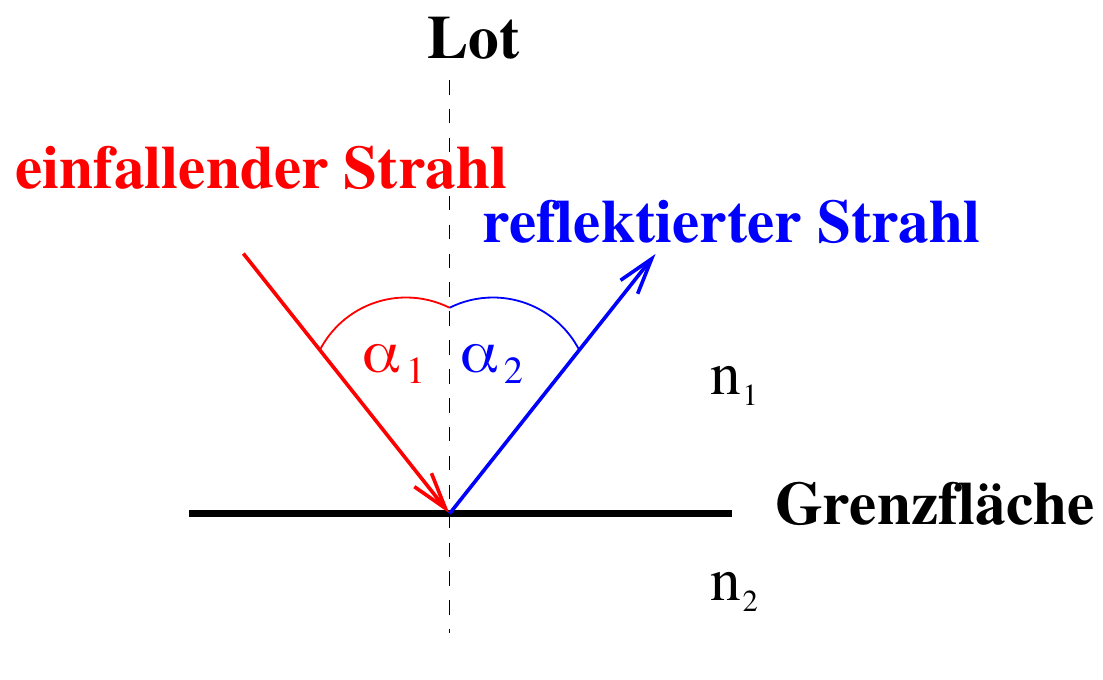
\includegraphics[scale = 0.3]{pictures/Reflexion.png}
    \caption{Reflexion eines Lichtstrahls. Quelle: \cite{AP01}}
    \label{fig:reflexion}
\end{figure}

\subsubsection*{Brechung}
\label{sec:brechung}
Die Ausbreitungsgeschwindigkeit von Licht hängt von dem Medium ab, in dem es sich bewegt. wechselt ein Lichtstrahl
nun an einer Grenzfläche das Medium, kommt es zur Brechung des Strahls, da sich die Ausbreitungsgeschwindigkeit
ändert. Dabei verhält sich das Verhältnis der Geschwindigkeiten zu den Winkeln des Lichtstrahls wie
\begin{equation}
    \frac{v_1}{v_2}=\frac{\sin\alpha}{\sin\beta}=\frac{n_2}{n_1}.
    \label{eqn:brechung1}
\end{equation}
Dabei wurde der Brechungsindex $n$ eingeführt, welcher als Materialeingenschaft den Zusammenhang \ref{eqn:brechung}
bestmöglich beschreibt. Die Brechung eines Lichtstrahls an einer Grenzfläche zwischen zwei Medien mit verschiedenen
Brechungsindizes ist in Abbildung \ref{fig:brechung} dargestellt.
\begin{figure}[H]
    \centering
    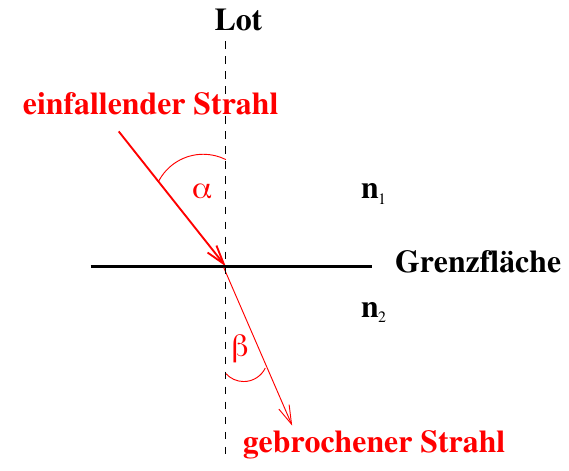
\includegraphics[scale = 0.5]{pictures/Brechung.png}
    \caption{Brechung eines Lichtstrahls. Quelle: \cite{AP01}}
    \label{fig:brechung}
\end{figure}
Der Brechungsindex von Luft liegt bei ca. $\num{1.000292}$ \cite{AP01} und ist daher für unsere Zwecke als $1$
zu setzen. Somit wird \ref{eqn:brechung1} für $n_1\approx1$ zu
\begin{equation}
    \frac{\sin\alpha}{\sin\beta}=n_2.
\end{equation} 
Die Ausbreitungsgeschwindigkeit von Licht in einem Medium hängt jedoch nicht nur von dem Brechungsindex des Mediums
ab, sondern auch von der Wellenlänge $\lambda$ des Lichtstrahls. Somit verändert sich auch das Brechungsverhalten.
Diese Abhängigkeit wird Disperion genannt und wird erneut in Kapitel \ref{sec:prisma} aufgegriffen. 

\subsubsection*{Reflexion und Transmission}
\label{sec:RefTrans}
Allgemein finden sowohl Reflexion als auch Brechung statt, wenn ein Lichtstrahl auf eine Grenzfläche zweier 
Medien trifft. Ein gewisser Anteil der Intensität $R$ wird an der Grenzfläche reflektiert und der restliche 
Teil der Intensität $T$ transmittiert durch die Grenzfläche und wird gebrochen. Da bei diesem Prozess die 
Summe der Intensität erhalten bleibt gilt
\begin{equation}
    R+T=1
\end{equation}
Wie groß nun die Intensität verteilt wird ist von den Materialien abhängig. In Abbildung \ref{fig:RefTrans}
sind die beiden Prozesse aus Abbildung \ref{fig:reflexion} und \ref{fig:brechung} zusammengetragen.
\begin{figure}[H]
    \centering
    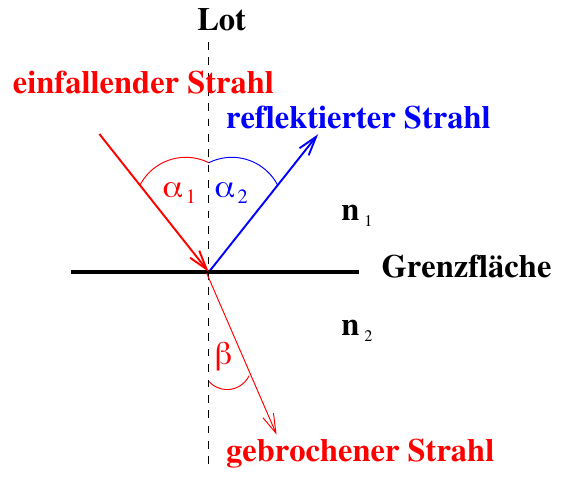
\includegraphics[scale = 0.5]{pictures/ReflexionTransmission.png}
    \caption{Reflexion und Transmission eines Lichtstrahls. Quelle: \cite{AP01}}
    \label{fig:RefTrans}
\end{figure}

\subsection{Beugung}
\label{sec:beugung}

\subsection{Prisma}
\label{sec:Prisma}